% !TeX spellcheck = en_GB
%\documentclass[handout]{beamer}\mode<presentation>{\usetheme{AMSCesenaPurpleAndGold}}
\documentclass[presentation]{beamer}\mode<presentation>{\usetheme{AMSCesenaPurpleAndGold}}
%%%%

\usepackage{sd-lab-building-linda}
%\usepackage{my-listings}
\usepackage{forloop}

\newcommand{\bs}[1]{\textbackslash{}#1}
\newcommand{\labN}{6}
\newcommand{\labGroup}{https://gitlab.com/pika-lab/courses/ds/ay2021}
\newcommand{\labRepo}{\labGroup/lab-\labN}

\title[L\labN{} -- Building \linda{}]{L\labN{} -- Building \linda{} from scratch}
%
\subtitle[SD]{Distributed Systems / Technologies}
%
\author[Ciatto \and Omicini]
{\emph{Giovanni Ciatto} \and Andrea Omicini\\
	\texttt{giovanni.ciatto@unibo.it \and andrea.omicini@unibo.it}}
%
\institute[DISI, Univ. Bologna]
{Dipartimento di Informatica -- Scienza e Ingegneria (DISI)\\\textsc{Alma Mater Studiorum} -- Universit{\`a} di Bologna a Cesena}
%
\date[A.Y. 2020/2021]{Academic Year 2020/2021}

\setbeamercovered{transparent}

\AtBeginSection{
	\begin{frame}[c]\frametitle{Outline}
		% 		\begin{multicols}{2}
		\tableofcontents[sectionstyle=show/shaded, subsectionstyle=hide/hide, subsubsectionstyle=hide/hide]
		% 		\end{multicols}
	\end{frame}
}

\AtBeginSubsection{
	\begin{frame}[c]\frametitle{Next in Line\ldots}
		\begin{multicols}{2}
			\small
			\tableofcontents[sectionstyle=show/shaded, subsectionstyle=show/shaded, subsubsectionstyle=hide/hide]
		\end{multicols}
	\end{frame}
}

\begin{document}

%\\\\\\\\\\\\\\\\\\\\\
\frame{\titlepage}
%\\\\\\\\\\\\\\\\\\\\\

\section{Motivation \& Goals}

\begin{frame}
\frametitle{Motivations}

\begin{itemize}
	\item So far, we have mostly focused on the \emph{structural} and \emph{behavioural} dimensions of software engineering (SE)

	\vfill

	\item It is now time to explore the \emph{interactive} dimension

	\vfill

	\item Interaction among agents can be modelled in several ways
	%
	\begin{itemize}
		\item and each model can be realised even more ways
	\end{itemize}

	\vfill

	\item Here we focus on the \alert{\linda{}} model, letting agents interact via \emph{tuple spaces}
	%
	\begin{itemize}
		\item very impactful model from the CS literature
		\item very central w.r.t. the field of Coordination
		\item very simple, yet very \emph{expressive}
		\item very didactic
	\end{itemize}

	\vfill

	\item Later, more complex sorts of \emph{interaction patterns} will be built on top of \linda{}

\end{itemize}

\end{frame}

\begin{frame}
	\frametitle{Lecture Goals}

	\begin{itemize}

		\item Become familiar with the \linda{} model in all its aspects

		\vfill

		\item Learn how to \alert{design \& build} a \linda{} implementation for multi-threaded applications in Java

		\vfill

		\item Learn how to derive an actual design out of an informal specification

		\vfill

		\item Learn how to recognise the many \emph{subtleties} of an informal specification

		\vfill

		\item Learn how \linda{} enables several \emph{interaction patterns} for agents

	\end{itemize}

\end{frame}

\subsection{About the practical activities}

\begin{frame}
	\frametitle{Lab \labN{} Repository on GitLab}

	\begin{itemize}
		\item Examples and exercises described in this lecture are provided by means of the following GitLab repository:
		%
		\begin{center}
			\url{\labRepo}
		\end{center}

		\vfill

		\item Clone it on your machine using Git
		%
		\begin{itemize}
		    \item[\$] \texttt{git clone \textit{<repo URL>}}
		\end{itemize}

		\vfill

		\item Even if a minimal environment simply relying on a text editor + Gradle is sufficient for this lab, we kindly suggest to import the cloned repository into some IDE, e.g. IntelliJ Idea or Eclipse
		%
		%
%		\begin{itemize}
%		    \item in case of problems in importing the project on IntelliJ, try to downgrade the gradle wrapper
%		    %
%		    \item[\$] \texttt{./gradlew wrapper \alert{--gradle-version \textit{4.8.1}}}
%		\end{itemize}

		\vfill

		\item In order to be able to submit your exercises, please ensure you requested access to the \href{\labGroup}{GitLab group of the course}
	\end{itemize}

\end{frame}

\section{Linda Recap}

%\subsection{Overview}

\begin{frame}%[allowframebreaks]
\frametitle{The \linda{} model}

\begin{itemize}
	\item The \linda{} model is built up of five main (sorts of) elements:
	%
	\begin{description}
		\item[Tuples] | structured information chunks (such as strings, records, dictionaries, or other kinds of \alert{data structures})

		\item[Templates] | compact notations for expressing sets of tuples adhering to the same pattern (e.g. regular expressions are templates w.r.t. strings).
		%
		Such patterns express some \alert{partial knowledge} about one or more tuple

		\item[Tuple Spaces] | unordered containers (i.e., \alert{multisets}) of tuples, which may evolve over time since tuples may be added or removed

		\item[Agents] (or ``Processes'', or ``Activities'') | pro-active entities which interact by writing, observing, or taking information from the tuple spaces

		\item[Primitives] | operations which can be performed by agents on tuple spaces, in order to manipulate or observe the information they contain
	\end{description}
\end{itemize}
\end{frame}

%\subsection{Primitives}

\begin{frame}%[allowframebreaks]
\frametitle{\linda{'s} primitives}
	\begin{itemize}
		\item The minimal set of \alert{primitives} according to the original \linda{'s} model comprehends the following ones:
		%
		\begin{description}
			\item[\texttt{out}] | let agents \alert{write} (or \alert{insert}) a tuple into a tuple space

			\item[\texttt{rd}] (shortcut for \alert{read}) | let agents know if a tuple matching a particular template \alert{exists} on a tuple space.
			%
			If it is the case, agents can also read the content of such a tuple

			\item[\texttt{in}] | let agents \alert{take} (or \alert{consume}) a tuple matching a particular template on a tuple space, if any
		\end{description}

		\item Other primitives will be considered in the future, but for the moment this is all we need

		\item Think about tuple spaces as \alert{collections}, about tuples as the the elements contained by such collections, and about primitives as the \alert{interface} of tuple spaces
	\end{itemize}
\end{frame}

%\subsection{The blackboard metaphor}

%\begin{frame}
%\frametitle{The blackboard metaphor}
%
%	\begin{enumerate}
%		\item You can imagine a tuple space as a \alert{blackboard}
%		%
%		\begin{center}
%			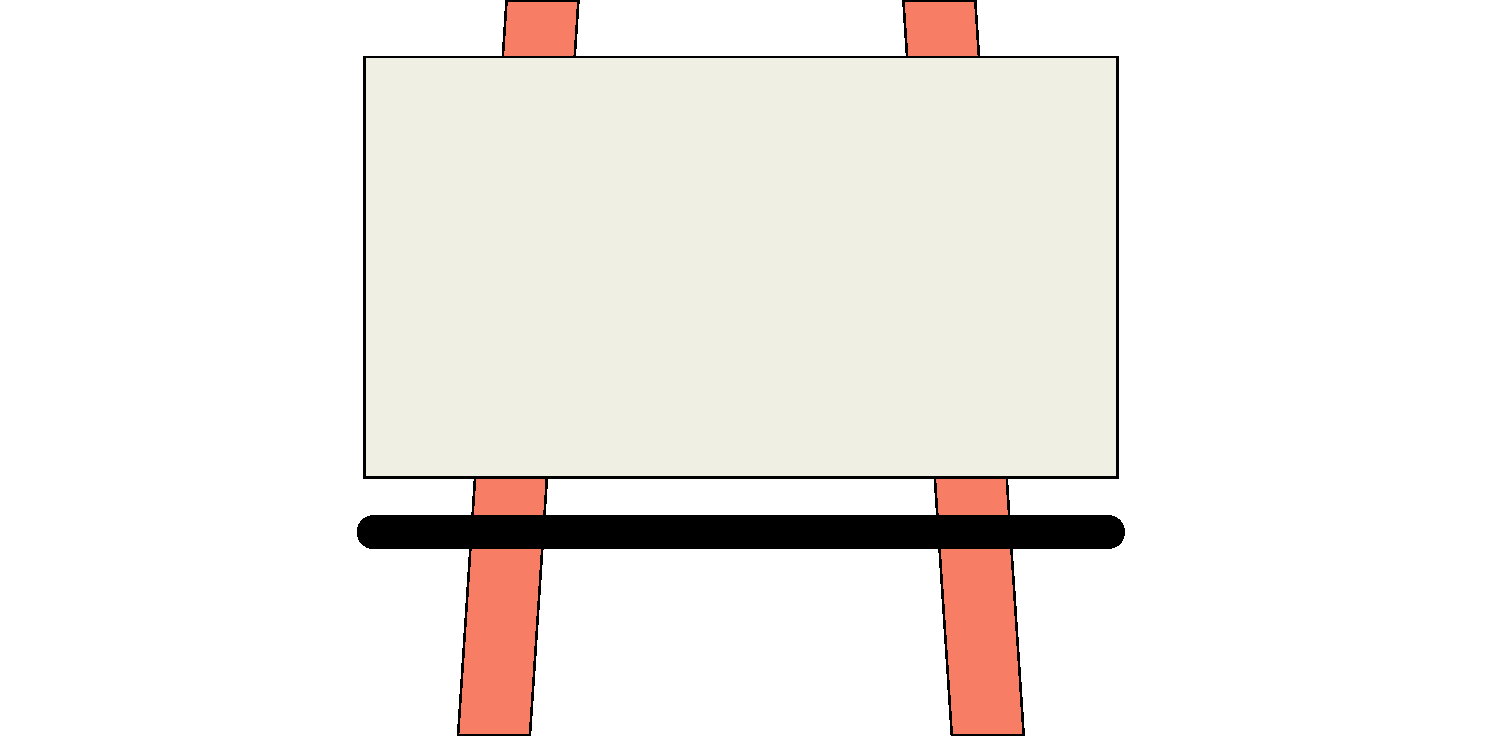
\includegraphics[width=\linewidth]{./img/blackboard.pdf}
%		\end{center}
%		%
%	\end{enumerate}
%
%\end{frame}
%
%\newcounter{imagenumber}
%
%\forloop{imagenumber}{1}{\value{imagenumber} < 4}{
%\begin{frame}
%\frametitle{The blackboard metaphor}
%
%	\begin{enumerate}\setcounter{enumi}{2}
%	    \item where agents can \alert{\texttt{write}} any sort of information---[i.e.] \alert{tuples}
%	    \begin{itemize}
%	        \item according to some \alert{representation} format of choice
%	        \item through primitive \alert{\texttt{out}}
%	    \end{itemize}
%		%
%		\begin{center}
%			\includegraphics[width=\linewidth]{./img/write-\arabic{imagenumber}.pdf}
%		\end{center}
%		%
%	\end{enumerate}
%
%\end{frame}
%}
%
%\forloop{imagenumber}{1}{\value{imagenumber} < 4}{
%\begin{frame}
%\frametitle{The blackboard metaphor}
%
%	\begin{enumerate}\setcounter{enumi}{3}
%
%	\item where agents can \alert{\texttt{read}} all information matching a particular \alert{template}
%	\begin{itemize}
%		\item according to some \alert{query} language of choice
%		\item through primitive \alert{\texttt{rd}}
%	\end{itemize}
%	%
%	\begin{center}
%		\includegraphics[width=\linewidth]{./img/read-\arabic{imagenumber}.pdf}
%	\end{center}
%	%
%	\end{enumerate}
%\end{frame}
%}
%
%\forloop{imagenumber}{1}{\value{imagenumber} < 4}{
%\begin{frame}
%\frametitle{The blackboard metaphor}
%
%	\begin{enumerate}\setcounter{enumi}{4}
%
%		\item or \alert{\texttt{take}} it, making it unaccessible for other agents
%		%
%		\begin{itemize}
%		    \item through primitive \alert{\texttt{in}}
%		\end{itemize}
%		%
%		\begin{center}
%			\includegraphics[width=\linewidth]{./img/take-\arabic{imagenumber}.pdf}
%		\end{center}
%	\end{enumerate}
%\end{frame}
%}

%\subsection{Semantics}

\begin{frame}%[allowframebreaks]
\frametitle{Semi-Formal notation}

	In what follows, we will use the following notation:
	%
	\vfill
	%
	\begin{itemize}
		\item Tuples are enumerated by \alert{$t$}, or $t_i$, so, r.g., $t_1 \neq t_2$, but $t_0 = t_0$
		%
		\begin{itemize}
			\item whereas $\mathbf{t}^*$ denotes a vector of tuples
		\end{itemize}

		\vfill

		\item Templates are enumerated by \alert{$\bar{t}$}, or $\bar{t}_i$. Notice that templates are a compact way to represent \alert{sets} of tuples
		%
		\begin{itemize}
			\item whereas $\bar{\mathbf{t}}^*$ denotes a vector of templates
		\end{itemize}

		\vfill

		\item Matching is written as \alert{$t \in \bar{t}$}, i.e., tuple $t$ matches template $\bar{t}$
		%
		\begin{itemize}
			\item unless stated otherwise, we implicitly assume the following notation: tuple $t$ matches template $\bar{t}$, tuple $t_1$ matches template $\bar{t_2}$, tuple $t_i$ matches template $\bar{t_i}$, and so on \ldots
		\end{itemize}

		\vfill

		\item Tuple Spaces are enumerated by \alert{$TS$}, or $TS_j$

		\vfill

		\item Agents are enumerated by \alert{$A$}, or $A_k$
	\end{itemize}

\end{frame}

\begin{frame}[fragile]
\frametitle{\linda{} Informal Semantics}
\label{linda-semantics}

	\begin{description}
		\item[Generative] | after an agent $A$ performs a \texttt{out($t$)} operation on some tuple space $TS$, tuple $t$ \alert{exists} regardless of $A$.
		%
		If agent $A$ terminates, crashes, or disconnects, $t$ will keep existing on $TS$

		\item[Associative] | tuples are \alert{accessed} (read or taken) in an associative way: instead of using a name, or an address, agents can specify \alert{templates} in order to access tuples

		\item[Suspensive] | whenever an agent $A$ invokes the \texttt{rd($\bar{t}$)} or \texttt{in($\bar{t}$)} over a particular template $\bar{t}$, on a particular tuple space $TS$, if not tuple $t$ matching $\bar{t}$ exists on $TS$, the operation is \alert{suspended} until $t$ is inserted into $TS$ by some agent performing a \texttt{out($t$)} operation

		\item[Non-deterministic] | whenever an agent $A$ invokes the \texttt{rd($\bar{t}$)} or \texttt{in($\bar{t}$)} operation, if more than one tuple $t$, $t'$, $t''$ exist matching  $\bar{t}$, one is read or taken  \alert{non-deterministically}

	\end{description}

\end{frame}


\section{\linda{} in Java}

\subsection{Abstract Design}

\begin{frame}%[allowframebreaks]
	\frametitle{Communication vs. Coordination Language}

	An actual designing of \linda{} involves the specification of two major aspects:

	\vfill

	\begin{block}{The \textbf{communication} language}
		\begin{itemize}
			\item dictating how \emph{tuples} and \emph{templates} are represented
			\item as well as \emph{matches} are computed among them
		\end{itemize}
	\end{block}

	\vfill

	\begin{block}{The \textbf{coordination} language}
		\begin{itemize}
			\item dictating which and how many \emph{primitives} are available for agents
		\end{itemize}
	\end{block}

\end{frame}

\begin{frame}%[allowframebreaks]
	\frametitle{Communication Language}

	To define a communication language, one should have an answer to the following questions:
	%
	\vfill
	%
	\begin{itemize}
		\item which sorts of \emph{information} should agents be able to manipulate?
		%
		\begin{itemize}
			\item[eg] numbers? vectors? text? objects? graphs? etc.
		\end{itemize}

		\vfill

		\item which sorts of \emph{data representation} formats should \linda{} support?
		%
		\begin{itemize}
			\item[eg] doubles? arrays? strings? XML? JSON? etc.
		\end{itemize}

		\vfill

		\item which \emph{information retrieval mechanism} is more adequate for the chosen format?
		%
		\begin{itemize}
			\item[eg] pattern matching? SQL? regular expressions? JSON Path? XPath?
		\end{itemize}

		\vfill

		\item how should \emph{templates} be represented to support the chosen format?

		\vfill

		\item given a tuple-template couple, how should \emph{a match} be computed?
	\end{itemize}

\end{frame}

\begin{frame}%[allowframebreaks]
	\frametitle{Coordination language}

	The \linda{} coordination language is composed by the \emph{canonical} primitives.
	%
	Yet, other primitives may be added to make the model address some specific issues:
	%
	\vfill
	%
	\begin{description}

		\item[utility] primitives (e.g. \alert{\texttt{set($\bar{\mathtt{t}}^*$)}}, \alert{\texttt{get()}}, \alert{\texttt{count()}}), while let agents overwrite, read, or count the whole content of a TS

		\vfill

		\item[predicative] primitives (e.g. \alert{\texttt{inp($\bar t$)}} and \alert{\texttt{inp($\bar t$)}}), which work as their canonical counterparts (i.e., \texttt{in($\bar t$)} and \texttt{rd($\bar t$)}) except they fail instead of suspending if no tuple matching $\bar t$ exists

		\vfill

		\item[``test for absence''] primitives (e.g. \alert{\texttt{no($\bar t$)}} and \alert{\texttt{nop($\bar t$)}}), which check if no tuple matching $\bar t$ exists, either suspending or failing in case at least a \emph{counterexample} exist

		\vfill

		\item[bulk] primitives (e.g. \alert{\texttt{out\_all($\bar{\mathtt{t}}^*$)}}, \alert{\texttt{in\_all($\bar t$)}}, and \alert{\texttt{rd\_all($\bar t$)}}) which let agents insert, consume, or read multiple tuples at a time
	\end{description}

	\vfill

\end{frame}

\subsection{Concrete Design}

\begin{frame}%[allowframebreaks]
	\frametitle{\linda{} as a Java interface}

	\begin{itemize}
		\item A TS can be easily conceived as an \alert{object} in the OOP sense

		\vfill

		\item which is generic in the type of tuples (i.e. \texttt{\alert{T}}) and templates (i.e. \texttt{\alert{TT}})

		\vfill

		\item where primitives return \alert{\texttt{CompletableFuture}s} to deal with suspension \& latency
	\end{itemize}

	\vfill

	\lstinputlisting[language=Java]{./code/TupleSpace.java}
\end{frame}

\begin{frame}%[allowframebreaks]
\frametitle{Where \texttt{Tuple}s and and \texttt{Template}s are simply:}

	\columsHH{
		\lstinputlisting[language=Java]{./code/Tuple.java}
	}{
		\lstinputlisting[language=Java]{./code/Template.java}
	}

	\begin{itemize}
		\item Tuples may be potentially anything
		%
		\begin{itemize}
			\item[eg] strings, objects, JSON files, XML files, logic terms, \ldots
		\end{itemize}

		\item Templates may be anything able to match a tuple, somehow
		%
		\begin{itemize}
			\item[eg] regular expressions, SQL, JsonPath, XPath, logic terms, \ldots
		\end{itemize}
	\end{itemize}

	\vfill

	\begin{block}{When designing some \linda{} implementation, you must decide}
		\begin{itemize}
			\item How to represent data (i.e. \alert{tuples})
			\item How to represent queries (i.e. \alert{templates})
			\item Which is the desired semantics for queries (i.e. the \alert{matching} mechanism)
		\end{itemize}
	\end{block}

\end{frame}

\subsection{Textual Tuple Spaces in Java}

\begin{frame}%[allowframebreaks]
\frametitle{Textual Tuple Spaces in Java -- Proof of Concept}

	We will implement the \texttt{TupleSpace} interface by means of the \texttt{\alert{Textual}Space} class, where:
	%
	\vfill
	%
	\begin{itemize}
		\item Strings are used as tuples, meaning that the \texttt{\alert{String}} class is used to reify tuples
	%
	\begin{itemize}
		\item[i.e.] \texttt{T $\rightarrow$ java.lang.\alert{String}}
	\end{itemize}

	\vfill

	\item Regular Expressions (regex) are used as templates, meaning that the \texttt{\alert{Pattern}} class is used to reify templates
	%
	\begin{itemize}
		\item[i.e.] \texttt{TT $\rightarrow$ java.util.regex.\alert{Pattern}}
		\end{itemize}

		\vfill

		\item The matching consists of \alert{deciding} whether a string matches a regex

		\vfill

		\item[!] If you are not practical with regex, you can acquire some experience or simply test your patterns with \url{https://regex101.com}
	\end{itemize}

\end{frame}

\begin{frame}
\frametitle{String as Tuples}

	\texttt{StringTuple} is just a \emph{wrapper} type for Java's \texttt{String}s:
	%
	\lstinputlisting[language=Java]{./code/StringTuple.java}

\end{frame}

\begin{frame}
\frametitle{Regex as Templates}

	\texttt{RegexTuple} is just an \emph{adapter}\footnote{\url{https://en.wikipedia.org/wiki/Adapter_pattern}} type for Java's \texttt{Pattern}s:
	%
	\lstinputlisting[language=Java]{./code/RegexTemplate.java}

\end{frame}

\begin{frame}
	\frametitle{\href{https://regex101.com/}{Regex101.com} -- Example}

	\begin{itemize}
		\item Could you say what's the meaning of the following regex?
		%
		\begin{center}\small
			\alert{\texttt{\bs{s}*to\bs{s}*:\bs{s}*"([A-Za-z ]+)",\bs{s}*from\bs{s}*:\bs{s}*"([A-Za-z ]+)"\bs{s}*}}
		\end{center}
		%
		\begin{center}
			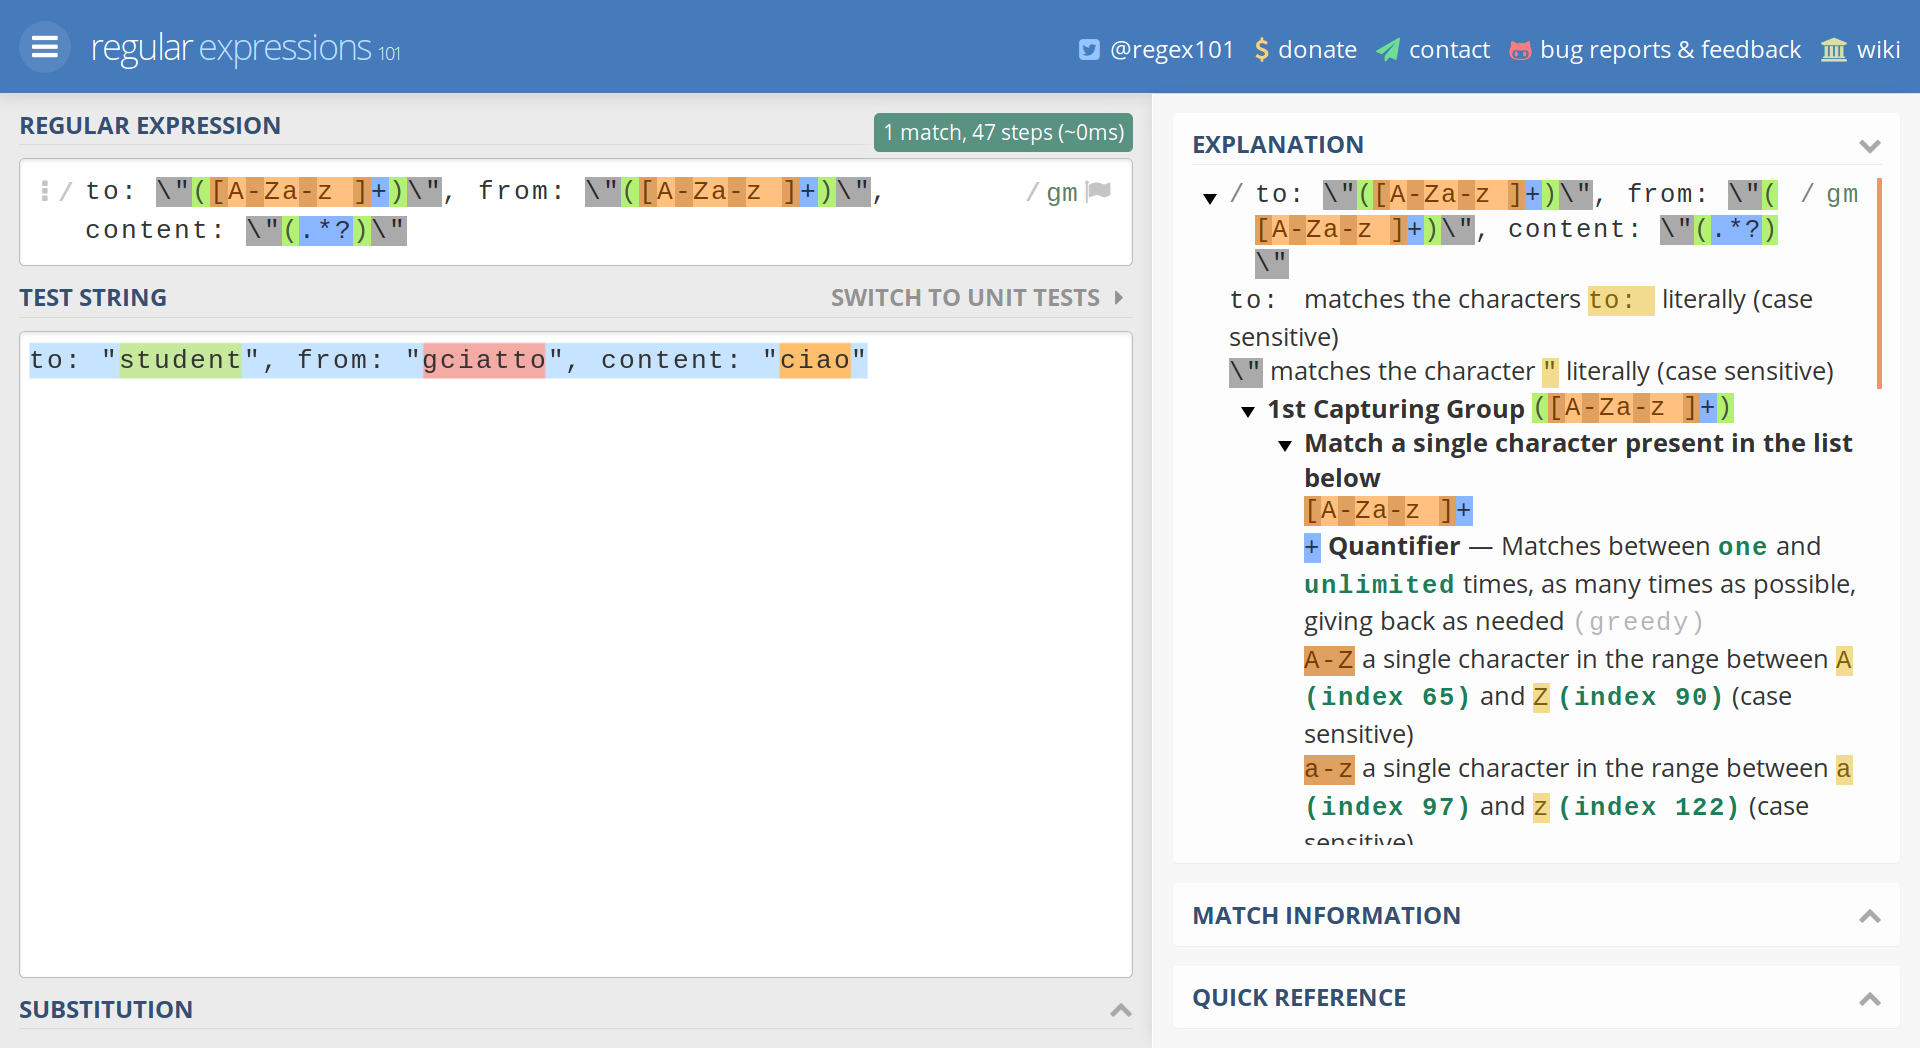
\includegraphics[width=.7\linewidth]{./img/regex101.png}
		\end{center}

		\item \url{https://regex101.com/r/2eU8aO/2} provides an interactive explanation of the regex above (on the right side)
		%
		\begin{itemize}
			\item you can test your regex on the fly against any input string
			\item consider inspecting the documentation of \href{https://docs.oracle.com/en/java/javase/14/docs/api/java.base/java/util/regex/Pattern.html}{\texttt{java.util.regex.\alert{Pattern}}}
		\end{itemize}

	\end{itemize}
\end{frame}

\section{Exercises (pt. 1)}

\startExercise

\subsection{Particular Communication Languages}

\begin{frame}[allowframebreaks]
	\frametitle{Exercise \currentExercise{} -- Particular Communication Languages}

	Use \href{https://regex101.com/}{Regex101.com} to practice with regex-based templates:

	\begin{block}{Service descriptors}
		\begin{itemize}
			\item Imagine strings represent \alert{service descriptors} in the form:
			%
			\begin{center}\ttfamily\small
				OutputType ServiceName ( InputType$_1$ , InputType$_2$ , $\ldots$ )
			\end{center}

			\item Define a regex for all service descriptors that:
			%
			\begin{enumerate}
				\item return an \texttt{int}
				\item accept a \texttt{long} as first input argument
				\item return a \texttt{double}, are named \texttt{sum}, and accept an arbitrary amount of \texttt{double}s as input
			\end{enumerate}
		\end{itemize}
	\end{block}

	\begin{block}{Messages}
		\begin{itemize}
			\item Imagine strings represent \alert{messages} in the form:
			%
			\begin{center}\ttfamily\small
				from: "Sender", to: "Receiver", content: "Payload"
			\end{center}

			\item Define a regex for all messages that:
			%
			\begin{enumerate}
				\item are directed towards \texttt{alice}
				\item have been sent by \texttt{bob}
				\item carry a payload which is either \texttt{ping} or \texttt{pong}
			\end{enumerate}
		\end{itemize}
	\end{block}

\end{frame}

\startExercise

\subsection{Text-based Tuple Spaces in Java}

\begin{frame}[allowframebreaks]
\frametitle{Exercise \currentExercise{} -- Textual Tuple Spaces in Java}

\begin{enumerate}
	\item Clone the initial source code from \url{\labRepo}

	\medskip

	\item Import the project into your favourite IDE as a Gradle project

	\medskip

	\item Inspect the provided code and try to figure out its purpose

	\medskip

	\item Notice that the project's \texttt{build.gradle.kts} file comes with some dependencies.
	%
	Try to figure out what they are and what's their purpose

	\medskip

	\item Notice that the project comes equipped with some tests.
	%
	Read them and try to understand them
\end{enumerate}

\lstinputlisting[language=Java]{./code/TextualSpace.java}

\framebreak

Activity:
%
\bigskip
%
\begin{itemize}

	\item Provide an implementation for the \texttt{TextualSpace} interface\ldots

	\bigskip

	\item \ldots such that the \alert{unit tests} in \alert{\texttt{TestTextualSpace}} class are satisfied
	%
	\begin{itemize}
		\item use them as usage examples
	\end{itemize}

	\bigskip

	\item The tuple space must work regardless of the particular \texttt{ExecutorService} it is initialised with

	\bigskip

	\item The provided implementation must adhere to the \alert{\linda{} semantics} described on slide \ref{linda-semantics}

%	\bigskip
%
%	\item[!] If you feel confident with these concepts you can start your exercise now.
%	%
%	Otherwise, just wait for the teacher's tutorial
\end{itemize}
\end{frame}

\begin{frame}
%\frametitle{Design of access primitives (i.e. \texttt{in} and \texttt{rd})}

\begin{center}
	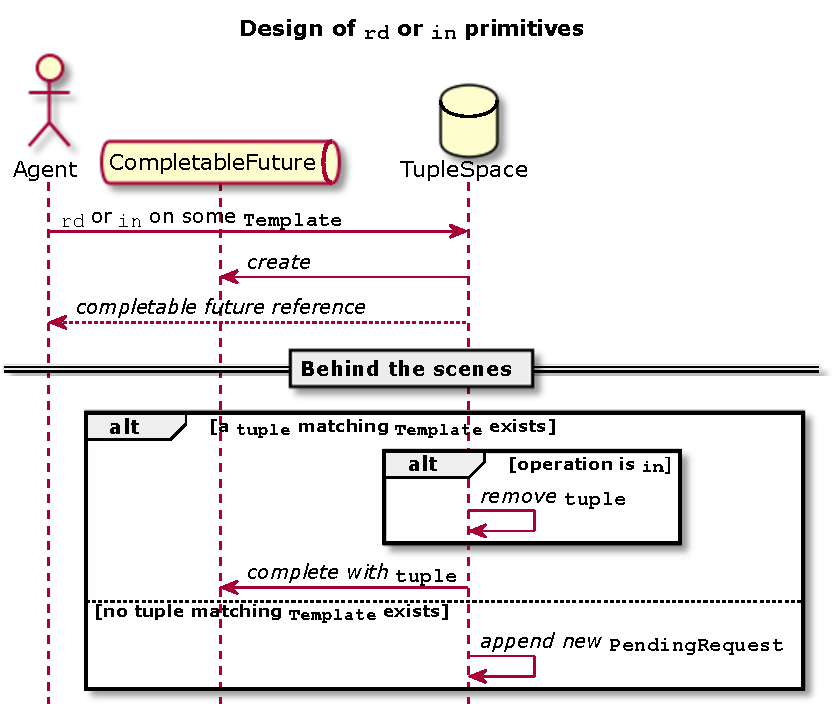
\includegraphics[width=.8\linewidth]{./img/rd-and-in-design.pdf}
\end{center}

\end{frame}

\begin{frame}
\frametitle{About pending requests}

\begin{itemize}
	\item Pending requests represent \alert{suspended} \texttt{in} and \texttt{rd} primitives to be eventually resumed by some \texttt{out}

	\vfill

	\item Each pending request carries the following information:
	%
	\begin{enumerate}
		\item the \alert{type} of the suspended primitive (i.e. either \texttt{in} or \texttt{rd})
		\item the \alert{template} the suspended primitive is waiting for
		\item some means to \alert{unlock} or resume the suspended primitive
		%
		\begin{itemize}
			\item[eg] the \texttt{\alert{CompletableFuture}} created when the suspended primitive has been invoked
		\end{itemize}
	\end{enumerate}

	\vfill

	\item[?] Can you tell \alert{why} all such information is needed?

	\vfill

	\item Have a look to the \texttt{sd.lab.linda.textual.impl.\alert{PendingRequest}} class for more details
\end{itemize}

\end{frame}

\begin{frame}

	\begin{center}
		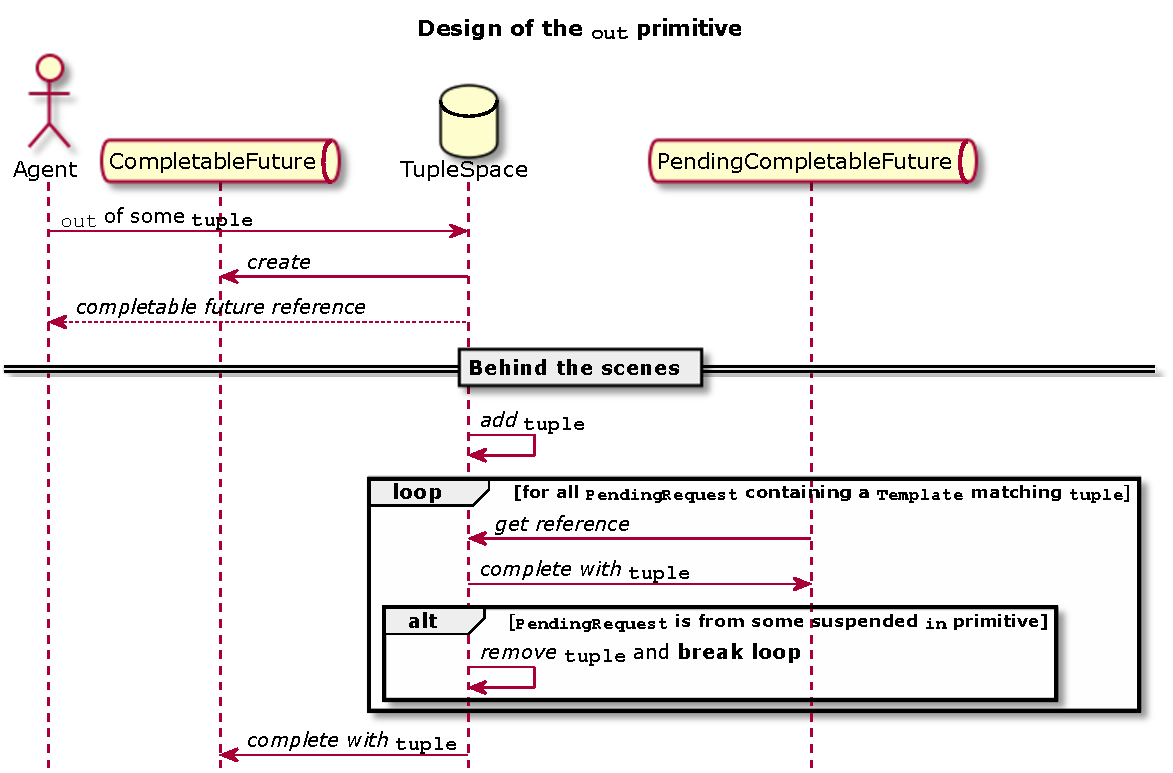
\includegraphics[width=.9\linewidth]{./img/out-design.pdf}
	\end{center}
	%
	\begin{itemize}
		\item[!] when should the \texttt{out}'s \texttt{CompletableFuture} completed? why?
	\end{itemize}

\end{frame}

\begin{frame}
\frametitle{General structure for primitives implementation}

\lstinputlisting[language=Java]{./code/GeneralPrimitiveImplementation.java}

\begin{itemize}
	\item[?] what's the purpose of the \texttt{\alert{synchronized}} keyword?
\end{itemize}

\end{frame}

%\begin{frame}[allowframebreaks]{Implementing the \texttt{rd} primitive}
%	\lstinputlisting[language=Java]{./code/TextualSpace_rd.java}
%\end{frame}
%
%\begin{frame}[allowframebreaks]{Implementing the \texttt{in} primitive}
%\lstinputlisting[language=Java]{./code/TextualSpace_in.java}
%\end{frame}
%
%\begin{frame}[allowframebreaks]{Implementing the \texttt{out} primitive}
%\lstinputlisting[language=Java]{./code/TextualSpace_out.java}
%\end{frame}

\begin{frame}{Exercise \currentExercise{} -- Go on by your self}
\begin{itemize}
	\item Try complete the implementation of \texttt{TextualSpace}

	\vfill

	\item There are two more utility primitives to be implemented in order for tests to work:
	%
	\begin{description}
		\item[\texttt{get}] | reads \alert{all} the tuples currently contained within the tuple space
		\item[\texttt{count}] | reads \alert{how many} tuples are currently contained within the tuple space
	\end{description}
	%
	Their functioning is essentially self-contained

\end{itemize}
\end{frame}

\subsubsection{Some Question}

\begin{frame}{Exercise \currentExercise{} -- Check your understanding}
Once you are done with the exercise, try to answer on the following questions (possibly, on the forum):
%
\vfill
%
\begin{enumerate}
	\item What makes \linda{} different from an ordinary (NoSQL?) database?

	\vfill

	\item What do we exactly mean by ``\alert{suspensive semantics}''? Which mechanism provides such feature?

	\vfill

	\item What do we exactly mean by ``\alert{non-determinism}''? Where / when did we address this feature in our exercise?

	\vfill

	\item Why do we adopt an asynchronous interface for the \texttt{\alert{out}} primitive as well, even if it is not suspensive?

\end{enumerate}
\end{frame}


%\section{Agents}
%
%\subsection{Agents as Threads}
%
%\begin{frame}{About agents}
%\begin{itemize}
%	\item Notice the \texttt{sd.lab.linda.\alert{Agent}} class
%
%	\vfill
%
%	\item It is extensively employed in testing control-flow-related issues
%	%
%	\begin{itemize}
%		\item[eg] \linda{}'s primitives
%	\end{itemize}
%
%	\vfill
%
%	\item We will extend this as well in the future, but for the moment it is a simple as this
%
%	\vfill
%
%	\item It is as simple as a thread executing some \alert{cyclic} behaviour
%
%\end{itemize}
%\end{frame}
%
%\begin{frame}[allowframebreaks]{Agents as threads}
%\lstinputlisting[language=Java]{./code/Agent.java}
%\end{frame}

\startExercise

\subsection{Predicative Primitives (Advanced)}

\begin{frame}[allowframebreaks]
	\frametitle{Exercise \currentExercise{} -- Predicative Primitives (Optional)}

	\begin{alertblock}{This is an \textbf{advanced} exercise}
		\begin{itemize}
			\item feel free to skip it
			\item try it if you are curious about making TS more practical
		\end{itemize}
	\end{alertblock}

	\bigskip

	Activity:
	%
	\medskip
	%
	\begin{enumerate}
		\item extend the \texttt{TupleSpace} interface with \alert{predicative} primitives
		%
		\begin{itemize}
			\item i.e. add the methods \texttt{inp} and \texttt{rdp}
		\end{itemize}

		\medskip

		\item implement these primitives in \texttt{TextualSpace}

		\medskip

		\item extend the suite \texttt{TestTextualSpace} to test the new primitives

	\end{enumerate}

\end{frame}

\startExercise

\subsection{Test for Absence Primitives (Advanced)}

\begin{frame}[allowframebreaks]
	\frametitle{Exercise \currentExercise{} -- Test for Absence Primitives (Optional)}

	\begin{alertblock}{This is an \textbf{advanced} exercise}
		\begin{itemize}
			\item feel free to skip it
			\item try it if you are curious about how advanced primitives work
		\end{itemize}
	\end{alertblock}

	\bigskip

	Activity:
	%
	\medskip
	%
	\begin{enumerate}
		\item extend the \texttt{TupleSpace} interface with \alert{test for absence} primitives
		%
		\begin{itemize}
			\item i.e. add the methods \texttt{no} and \texttt{nop}
		\end{itemize}

		\medskip

		\item implement these primitives in \texttt{TextualSpace}

		\medskip

		\item extend the suite \texttt{TestTextualSpace} to test the new primitives

	\end{enumerate}

\end{frame}

\section{Mediating Agents' Interaction}

\begin{frame}
\frametitle{Perspective}

	\begin{block}{What are now capable of}
		\begin{itemize}
			\item[$\checkmark$] instantiating several \alert{agents}, each one carrying on several \alert{behaviours}
			\item[$\checkmark$] instantiating several \alert{tuple spaces}
			\item[$\checkmark$] let one or more \alert{Java threads} manipulate those tuple spaces
			%
			\begin{itemize}
				\item via \linda{} primitives as method calls
			\end{itemize}
		\end{itemize}
	\end{block}

	\vfill

	\begin{alertblock}{What are we missing}
		\begin{itemize}
			\item[$\times$] lettings agents manipulate tuple spaces \alert{via behaviours}
			\item[$\times$] lettings agents \alert{exchange messages} through tuple spaces
			\item[$\times$] lettings agents \alert{interact} over the network
		\end{itemize}
	\end{alertblock}

\end{frame}

\subsection{Mixing Tuple Spaces and Agents}

\begin{frame}
	\frametitle{Injecting Tuple Spaces into our Agent framework}

	\begin{alertblock}{Focus on}
		\begin{itemize}
			\item[$\rightarrow$] lettings agents manipulate tuple spaces \alert{via behaviours}
		\end{itemize}
	\end{alertblock}

	\pause

	\begin{exampleblock}{Main idea}
		\begin{itemize}
			\item let all agents from the same environment access a \alert{shared} pool of tuple spaces
			\item endow agents with ad-hoc behaviour types to exploit \linda{} primitives
		\end{itemize}
	\end{exampleblock}

\end{frame}

\begin{frame}[allowframebreaks]
	\frametitle{Extending the Environment}

	\begin{alertblock}{Focus on}
		\begin{itemize}
			\item[$\rightarrow$] lettings agents manipulate tuple spaces \alert{via behaviours}
			%
			\begin{itemize}
				\item[$\rightarrow$] let all agents from the same environment access a \alert{shared} pool of tuple spaces
			\end{itemize}
		\end{itemize}
	\end{alertblock}

	\bigskip

	Suppose each \texttt{Environment} exposes a method to let agents access \texttt{TextualSpace} instances:
	%
	\lstinputlisting[language=Java]{./code/Environment.java}

	Intended usage:
	%
	\medskip
	%
	\begin{itemize}
		\item agents can always access their environments via their \texttt{getEnvironment()} method

		\medskip

		\item they can always access the tuple space named \alert{\texttt{"tsName"}} through:
		%
		\begin{center}\ttfamily
			getEnvironment().getTextualSpace(\alert{"tsName"})
		\end{center}

		\medskip

		\item if two or more agents access the same tuple space name, they get the \alert{same} instance
		%
		\begin{itemize}
			\item thus tuple spaces are \alert{shared} among agents
		\end{itemize}

		\medskip

		\item if a tuple space name has never been accessed, the corresponding tuple space is created \alert{on the fly} upon first access

	\end{itemize}

\end{frame}

\begin{frame}[allowframebreaks]
	\frametitle{Extending the Available Behaviours}

	\begin{alertblock}{Focus on}
		\begin{itemize}
			\item[$\rightarrow$] lettings agents manipulate tuple spaces \alert{via behaviours}
			%
			\begin{itemize}
				\item[$\checkmark$] let all agents from the same environment access a \alert{shared} pool of tuple spaces
				\item[$\rightarrow$] endow agents with ad-hoc behaviour types to exploit \linda{} primitives
			\end{itemize}
		\end{itemize}
	\end{alertblock}

	\framebreak

	Suppose the \texttt{Behaviour} hierarchy is extended as follows:
	%
	\begin{center}
		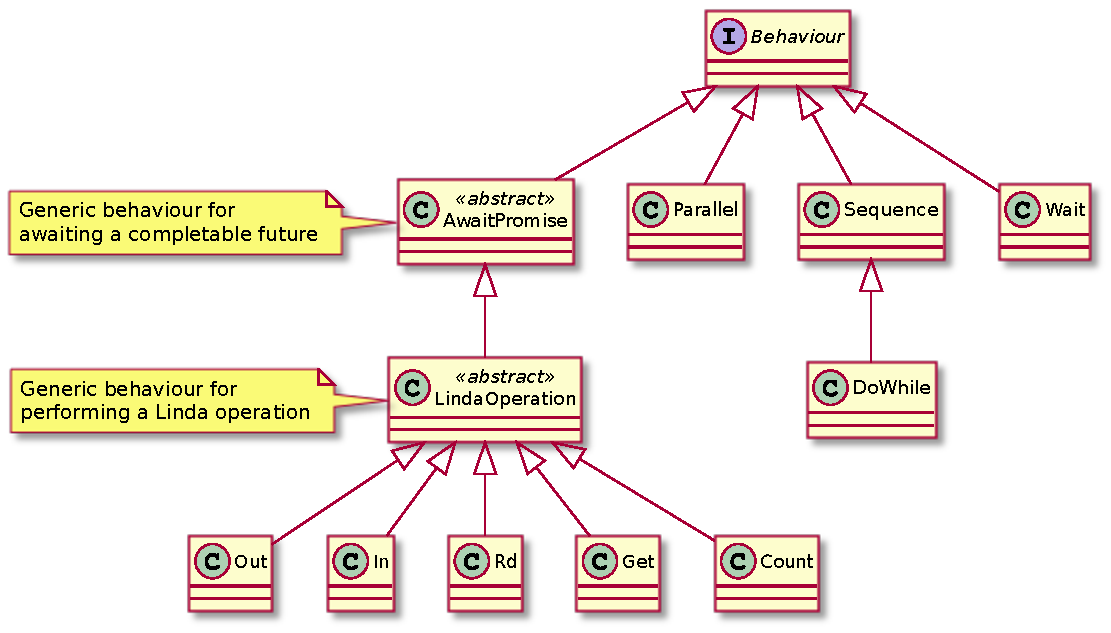
\includegraphics[width=.8\linewidth]{./img/classes-overview.pdf}
	\end{center}

	\framebreak

%	Design rationale:
%	%
%	\medskip
%	%
	\begin{itemize}
		\item \texttt{Out}, \texttt{In}, etc. are \alert{behaviours} aimed at letting an agent perform the corresponding \linda{} operation on some tuple space, given its name
		%
		\begin{itemize}
			\item in a \alert{synchronous} way, w.r.t. the behaviour
			\item meaning that the behaviour is \alert{paused} after the primitive \emph{invocation}$\ldots$
			\item $\ldots$ and resumed after its \emph{completion}
			\item yet, the agent may execute \emph{other} behaviours in the meanwhile
		\end{itemize}

		\medskip

		\item \texttt{LindaOperation} is the abstract behaviour letting an agent perform \alert{any} \linda{} operation on some tuple space, given its name
		%
		\begin{itemize}
			\item in a \alert{synchronous} way, w.r.t. the behaviour
		\end{itemize}

		\medskip

		\item \texttt{AwaitPromise} is the abstract behaviour letting an agent await the completion of \alert{any} \texttt{CompletableFuture}
		%
		\begin{itemize}
			\item in a \alert{synchronous} way, w.r.t. the behaviour
			\item in a \alert{non-blocking} way, w.r.t. the agent
			\item[!] as all \linda{} primitives rely on \texttt{CompletableFuture}s in our implementation, this is where most of the complexity lies
		\end{itemize}
	\end{itemize}

\end{frame}

\section{Exercises (pt. 2)}

\startExercise

\subsection{\linda{} Primitives as Behaviours}

\begin{frame}[allowframebreaks]
	\frametitle{Exercise \currentExercise{} -- \linda{} Primitives as Behaviours}

	Activity:
	%
	\bigskip
	%
	\begin{itemize}

		\item Provide an implementation for the classes: \texttt{AwaitPromise}, \texttt{Out}, \texttt{In}, etc.

		\bigskip

		\item \ldots such that the \alert{unit tests} in \alert{\texttt{TestAgentWithTupleSpaces}} class are satisfied
		%
		\begin{itemize}
			\item use them as usage examples
		\end{itemize}

		\bigskip

		\item More details about the to-be-implemented behaviours are provided in the next slides

		\bigskip

		\item Notice that most tests relies on two or more behaviours
		%
		\begin{itemize}
			\item thus, you may have to implement several behaviours before tests can pass
		\end{itemize}
	\end{itemize}

\end{frame}

\subsubsection{Awaiting Promises}

\begin{frame}[allowframebreaks]
	\frametitle{Exercise \currentExercise{} -- The \texttt{AwaitPromise} Behaviour}

	\begin{block}{The \texttt{AwaitPromise\textit{<T>}} behaviour}
		\begin{itemize}
			\item it waits for some \texttt{CompletableFuture\textit{<T>}} to be \alert{completed}, without blocking the agent
			%
			\begin{itemize}\small
				\item this is not used directly, but it is enabling for other primitives
			\end{itemize}
		\end{itemize}
	\end{block}

	\framebreak

	\begin{columns}
		\begin{column}{.8\linewidth}
			\begin{exampleblock}{\texttt{AwaitPromise\textit{<T>}} -- Design Rationale (pt 1)}
				\begin{itemize}
					\item It is an \textbf{abstract}, \alert{state\emph{ful}} and \alert{atomic} behaviour
					%
					\begin{itemize}
						\item it is stateful because it has several \alert{phases}
						\item[$\rightarrow$] we need to override the \texttt{\alert{deepClone()}} method \textbf{in sub-classes}
					\end{itemize}

					\medskip

					\item It aims at letting agents use \alert{\texttt{CompletableFuture}s} within behaviours
					%
					\begin{itemize}
						\item[why?] remember all those \texttt{CompletableFuture}s from the \alert{\texttt{TupleSpace}} interface?
					\end{itemize}

					\medskip

					\item It can be conceived as a FSA ranging through 4 states (a.k.a. \alert{phases})
					%
					\begin{itemize}
						\item FSA represented on the right
					\end{itemize}

				\end{itemize}
			\end{exampleblock}
		\end{column}
		\begin{column}{.18\linewidth}
			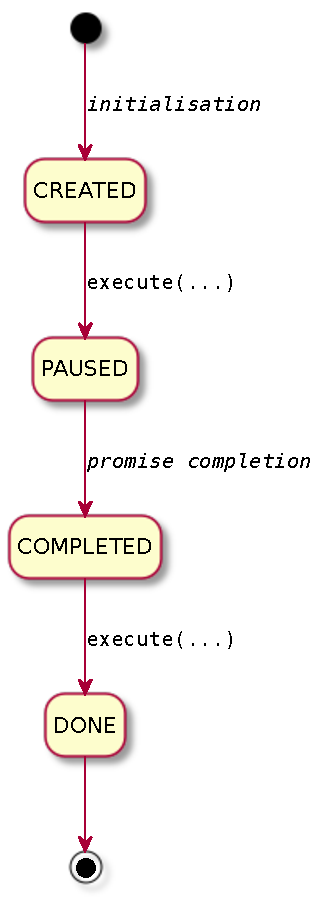
\includegraphics[width=\linewidth]{img/AwaitFSA.pdf}
		\end{column}
	\end{columns}

	\framebreak

	\begin{exampleblock}{\texttt{AwaitPromise\textit{<T>}} -- Design Rationale (pt 2)}
		\begin{itemize}
			\item It exposes 2 callbacks to be overridden by users:
			%
			\begin{description}\small
				\item[\texttt{invokeAsync(\ldots)}] returning the \texttt{CompletableFuture\textit{<T>}} this behaviour should wait for
				\item[\texttt{onResult(\ldots)}] callback to be invoked when the \texttt{CompletableFuture} is completed
			\end{description}

			\medskip

			\item When the \texttt{execute(...)} is firstly run, it adds an handler intercepting the \texttt{CompletableFuture}'s completion
			%
			\begin{itemize}
				\item after that, the current behaviour must be \alert{paused}
				\item it must be resumed when the \texttt{CompletableFuture} is completed
			\end{itemize}

			\medskip

			\item The $2^{nd}$ time the \texttt{execute(...)} is run must be after the \texttt{CompletableFuture} completion
			%
			\begin{itemize}
				\item this time, it must invoke the \texttt{onResult(...)} callback
				\item only then the \texttt{Await} behaviour can terminate
			\end{itemize}

		\end{itemize}
	\end{exampleblock}

\end{frame}

\startExercise

\subsection{Message Passing through \linda{}}

\begin{frame}[allowframebreaks]
	\frametitle{Exercise \currentExercise{} -- Message Passing through \linda{}}

	\begin{alertblock}{This is an \textbf{unconstrained} exercise}
		\begin{itemize}
			\item you are free to design your solution as you prefer
			\item no test is provided: testing is up to you
		\end{itemize}
	\end{alertblock}

	\bigskip

	\begin{alertblock}{This is a \textbf{mandatory} exercise}
		\begin{itemize}
			\item your solution will be inspected during lab activity verification
			\item you will be asked to discuss your solution
			\item collaboration and discussion with your colleagues (on the forum) is allowed
			\item asking for help on the forum is allowed
		\end{itemize}
	\end{alertblock}

	\framebreak

	\begin{block}{\textbf{Goal}}
		\begin{itemize}
			\item Let agents \emph{communicate} via message-passing
			\item Realise message passing \alert{on top} of \linda{}
		\end{itemize}
	\end{block}

	\begin{block}{How}
		\begin{enumerate}
			\item Endow agents with 2 more behaviour types: \alert{\texttt{Send}} and \alert{\texttt{Receive}}
			%
			\begin{itemize}
				\item \texttt{Send} may extend / exploit \texttt{Out}
				\item \texttt{Receive} may extend / exploit \texttt{In}
				\item Messages should be implemented as \texttt{StringTuple}s
				\item \texttt{TextualSpace}s may be exploited as \alert{inboxes}
			\end{itemize}
			\item Design your own solution, implement it, \textbf{and test it}
			%
			\begin{itemize}
				\item tests are the only thing proving your solution works
				\item[!] \textbf{tests are part of the exercise and will be assessed}
			\end{itemize}
		\end{enumerate}
	\end{block}

	\begin{exampleblock}{Subtleties}
		\begin{itemize}
			\item Each agent should only be able to receive messages \alert{directed towards it}
			\item An agent may be willing to \alert{select} messages according to the sender or the content, if more messages are available
		\end{itemize}
	\end{exampleblock}
\end{frame}

\startExercise

\subsection{Dining Philosophers (Advanced)}

\begin{frame}[allowframebreaks]
	\frametitle{Exercise \currentExercise{} -- Dining Philosophers (Optional)}

	\begin{alertblock}{This is an \textbf{advanced} exercise}
		\begin{itemize}
			\item feel free to skip it
			\item try it if you are curious about using TS in a \alert{multi-}agent scenario
		\end{itemize}
	\end{alertblock}

	\bigskip

	\begin{alertblock}{This is an \textbf{unconstrained} exercise}
		\begin{itemize}
			\item you are free to design your solution as you prefer
			\item no test is provided: testing is up to you
		\end{itemize}
	\end{alertblock}

	\bigskip

	\begin{block}{\textbf{Goal}}
		\begin{itemize}
			\item Implement a simple MAS involving $N \geq 3$ \alert{dining philosophers}
			\item Use \linda{} tuples to model \& implement chops
			\item Use \linda{} primitives to manipulate chops
			\item Provide a \alert{deadlock-free} implementation
		\end{itemize}
	\end{block}

\end{frame}

%=======================================================================
\section*{}
%===============================================================================

%\\\\\\\\\\\\\\\\\\\\\
\frame{\titlepage}
%\\\\\\\\\\\\\\\\\\\\\

%%===============================================================================
%\section*{\refname}
%%===============================================================================
%
%%\\\\\\\\\\\\\\\\\\\\\
%%%%%
%%\begin{frame}[t,allowframebreaks]\scriptsize
%\begin{frame}[c]\footnotesize
%\frametitle{\refname}
%\bibliographystyle{apalike}
%\bibliography{sd-lab-building-linda}
%\end{frame}
%%\\\\\\\\\\\\\\\\\\\\\

%%%%%%%%%%%%%%%%%%%%%%%%%%%%%%%%%%%%%%%%%%%%%%%%%%%%%%%%%%%%%%%%%%%%%%%%%%%%%%%
\end{document}
%%%%%%%%%%%%%%%%%%%%%%%%%%%%%%%%%%%%%%%%%%%%%%%%%%%%%%%%%%%%%%%%%%%%%%%%%%%%%%%%

